
\documentclass[11pt]{article}

\usepackage[papersize={210mm,297mm},left=25mm,right=25mm,top=30mm,bottom=30mm]{geometry}


\usepackage[hangul]{kotex}

\usepackage{iftex}
\ifPDFTeX
  \usepackage{dhucs-nanumfont}
\else\ifXeTeX
  \setmainhangulfont[Ligatures=TeX]{HCR Batang LVT}
  \setsanshangulfont[Ligatures=TeX]{HCR Dotum LVT}
\else\ifLuaTeX
  \setmainhangulfont[Ligatures=TeX]{HCR Batang LVT}
  \setsanshangulfont[Ligatures=TeX]{HCR Dotum LVT}
\fi\fi\fi


\usepackage{tikz}
\usepackage{tikz-3dplot}

\usepackage{graphicx}


\renewcommand*\thesection{\Roman{section}}


\renewcommand{\abstractname}{초록}

\makeatletter
\renewcommand\section{\@startsection {section}{1}{\z@}%
                                   {-3.5ex \@plus -1ex \@minus -.2ex}%
                                   {2.3ex \@plus.2ex}%
                                   {\normalfont\large\sffamily\bfseries}}

\renewcommand{\thesubsection}{\@arabic\c@subsection.\hspace*{-0.5em}}


  \renewenvironment{abstract}{%
      \if@twocolumn
        \section*{\abstractname}%
      \else
        %\small
        \begin{center}%
          {\large\sffamily\bfseries 초록\vspace{-.0em}\vspace{\z@}}%
        \end{center}%
        \quotation
      \fi}
      {\if@twocolumn\else\endquotation\fi}



\renewenvironment{thebibliography}[1]
     {\section{\refname}%
      \@mkboth{\MakeUppercase\refname}{\MakeUppercase\refname}%
      \list{\@biblabel{\@arabic\c@enumiv}}%
           {\settowidth\labelwidth{\@biblabel{#1}}%
            \leftmargin\labelwidth
            \advance\leftmargin\labelsep
            \@openbib@code
            \usecounter{enumiv}%
            \let\p@enumiv\@empty
            \renewcommand\theenumiv{\@arabic\c@enumiv}}%
      \sloppy
      \clubpenalty4000
      \@clubpenalty \clubpenalty
      \widowpenalty4000%
      \sfcode`\.\@m}
     {\def\@noitemerr
       {\@latex@warning{Empty `thebibliography' environment}}%
      \endlist}



\def\advisor#1{\gdef\@advisor{#1}}
\def\@advisor{\@latex@warning@no@line{No \noexpand\advisor given}}
\def\school#1{\gdef\@school{#1}}
\def\@school{\@latex@warning@no@line{No \noexpand\school given}}



\renewcommand\maketitle{\begin{titlepage}%
  \let\footnotesize\small
  \let\footnoterule\relax
  \let \footnote \thanks
  \null\vfil
  \vskip 60\p@
  \begin{center}%
    {\LARGE \@title \par}%
    \vskip 3em%
    {\large
     \lineskip .75em%
      \begin{tabular}[t]{c}%
        \@author
      \end{tabular}\par}%
      \vskip 1.5em%
    {\large \begin{tabular}[t]{c}\@date \end{tabular}\par}%       % Set date in \large size.
      \vskip 1.5em%
{\large
     \lineskip .75em%
      \begin{tabular}[t]{c}%
\@school   \and         \@advisor
      \end{tabular}\par}

  \end{center}\par
  \@thanks
  \vfil\null
  \end{titlepage}%
  \setcounter{footnote}{0}%
  \global\let\thanks\relax
  \global\let\maketitle\relax
  \global\let\@thanks\@empty
  \global\let\@author\@empty
  \global\let\@date\@empty
  %\global\let\@title\@empty
  \global\let\title\relax
  \global\let\author\relax
  \global\let\date\relax
  \global\let\and\relax
  \global\let\@advisor\@empty
  \global\let\advisor\relax
}





\makeatother


\usepackage{amsmath,amssymb,amsthm}
\usepackage{longtable}



\newtheorem{lemma}{보조정리}
\newtheorem{corollary}{따름정리}
\newtheorem{theorem}{정리}


\usepackage{fancyvrb}


\renewcommand{\proofname}{증명\quad}


\title{Cutting Problem of Simple Closed Curve in Single-vertex Curved Origami}  
\date{2014년 0월 0일} 
\school{서울과학고등학교}
\author{2816 최익한 \and 2712 정종욱} 
\advisor{지도교사 송원택}



%\usepackage{braids}


\usepackage{mflogo}

\usepackage{url}

\begin{document}
\thispagestyle{empty}
\maketitle





\begin{center}\huge\bfseries
\makeatletter\@title\makeatother
\end{center}
\vspace*{50mm}
\begin{abstract}\noindent
이 연구에서 vertex가 하나인 curved origami로의 fold-and-cut theorem의 확장 정리를 증명하였다.
\end{abstract}


\bigskip
\section{서론} 
Origami(折り紙)는 종이접기로 만드는 예술을 총칭하는 단어이며 수학에서는 종이를 접는 것으로부터 고안된 foldability나 수학적 방정식을 푸는데 이용하는 이론 등을 포괄하는 수학분야의 의미로 쓰인다. 역사적으로 1893년 T. Sundara Rao에 의해 기하학적 construction을 증명하는데 종이접기를 사용하는 것이 제시되었고 20세기 Margharita P. Beloch, R C Yeates, Jacques Justin 등에 의해 고전적 origami construction인 Huzita-Hatori axioms가 완성되었다. 1989년 'International Metting of Origami Science and Technology'가 이탈리아에서 열린 후 이 분야에서 꾸준한 연구가 이루어지고 있으며 최근에는 T. Hull, T. Tachi 등에 의해 추상대수적 개념으로의 확장이나 건축학과 밀접한 관련을 가지며 디자인에 관한 연구도 활성화 되어 있다. \cite{4,5,7,8} 연구의 방법론으로 미분기하학이나 복소수 및 사원수가 동원되는 등의 창의적인 연구결과도 보고되고 있다. \cite{2,3,9}
수학 분야로서의 Origami에서 제시되는 대표적인 문제들로 flat, rigid, curved, wet 등의 구체적인 조건이 붙어 종이로 원하는 모양을 접을 수 있는가에 관한 foldability를 조사하는 문제, Huzita-Hatori axioms과 같이 대수적, 기하적으로 정의되는 construction의 성질을 구하는 문제, 비록 해결되었지만 종이를 접은 후 직선으로 자른 모양에 대한 fold-and-cut Theorem 등이 있다.
Origami의 construction은 흔히 밖으로 접은 선(Mountain crease)과 안으로 접은 선 (Valley crease), 그리고 꼭짓점(vertex)으로 이루어진 crease pattern으로 나타내는 경우가 많다. Crease pattern으로부터 foldability를 구하는 문제는 다음 Lemma로써 증명되었다.


\begin{figure}
\centering
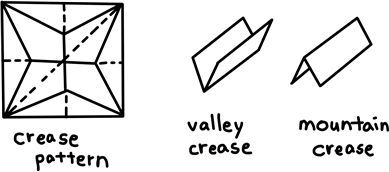
\includegraphics{1.png}
\caption{crease pattern, valley crease, mountain crease}
\end{figure}


\begin{lemma}
다음 네 가지 조건을 만족하는 crease pattern을 flat-foldable하다고 한다.
\\ $(1)$ 주어진 crease pattern이 two-colorable하다.
\\ $(2)$ $(Maekawa)$ 임의의 점에서 mountain crease의 수를 $M$, valley crease의 수를 $V$이라 할 때 $|M-V|=2$이다.
\\ $(3)$ $(Kawasaki)$ 임의의 점에서 모든 홀수$(짝수)$ 번째 각들의 합은 180도이다.
\\ $(4)$ 종이는 접힌 선을, 즉 자기 자신을 관통할 수 없다.
\end{lemma}


한 꼭짓점에 대하여 성립하는 flat-foldability를 local flat-foldability라 하며 여러 꼭짓점에 대하여 모두 성립하는 것을 global flat-foldability라 한다. 주어진 crease pattern을 보고 flat-foldable한지 조사하는 문제에 대하여 local flat-foldability는 위의 보조정리에 의해 완성되었지만 global flat-foldability는 NP-complete임이 증명되어 있다. \cite{1}
\\

표준좌표계로 $(s,t)$를 가지는 2차원 유클리드 공간 ${\mathbb R}^2$의 열린 집합 $U$와 $C^\infty$ 변환 $f:U\to {\mathbb R}^3$가 $U$ 안의 모든 점에서 $\frac{\partial f}{\partial s} \times \frac{\partial f}{\partial t} \ne 0 $일 때, 이 변환의 상 $M=f(U)$를 유클리드 공간 ${\mathbb R}^3$ 안에 있는 곡면(surface)이라고 하며 $f$를 곡면 $M$의 매개변수사상(patametrization)이라 한다. 곡면 $M$ 위의 점 $p$를 하나 고정하고 이 점에서 곡면에 수직한 법선벡터 $\nu$를 생각한 다음 곡면에 접하는 접벡터를 $T$라 하여 $T,\nu$를 포함하는 평면을 $N(T,\nu)$로 나타내고 법평면(normal plane)이라 한다. 이 법평면은 순서좌표축 $( T,\nu)$가 양의 방향성을 가지도록 좌표계가 설정되어 있는 평면이다. 매끄러운 곡선이 되는 공통부분집합 $\gamma_T = M\cap N(T,\nu)$에서 평면곡선에 관한 부호를 가지는 곡률(signed curvature)을 구하여 $T$방향의 법선 곡률(normal curvature)이라 하고 $\kappa (p,T)$로 나타낸다. 모든 접벡터 $T$에 대하여 $\kappa(p,T)$의 값이 모두 같은 점을 구면형(umbilic)이라 한다. \cite{10}


\begin{theorem}
$(Euler)$ 곡면 $M$ 위의 점 $p$가 구면형이 아니라고 할 때 법선 곡률의 최댓값 $\kappa_{\max}$를 주는 단위접선벡터 $T_{\max}$와 곡률의 최솟값 $\kappa_{\min}$을 주는 단위접선벡터 $T_{\min}$은 정확히 하나씩 존재하며 두 접벡터 $T_{\max}$와 $T_{\min}$은 수직이다. 또한 점 $p$의 임의의 접벡터 $T$가 $T_{\max}$와 이루는 각의 크기를 $\theta$라 하면 다음과 같은 식이 성립한다.


\begin{equation}
\kappa (p,T)=\kappa_{\max} \cos ^2 \theta+\kappa_{\min} \sin ^2 \theta. \nonumber
\end{equation}

\end{theorem}



이 때 최대, 최소 법선곡률의 값을 주요곡률(principle curvature)이라 하고 주요곡률을 주는 접벡터의 방향을 주요곡률방향이라 한다. 제 2 기본형식(Gauss' second fundamental form)을 행렬표현으로 나타냈을 때 이 행렬의 행렬식으로 표현되는 가우스 곡률은 $\kappa_{\max} \kappa_{\min}$의 값과 같다고 알려져 있다.


\begin{theorem}
(Gauss' Theorema Egregium) 만일 한 곡면이 다른 곡면의 isometry 관계에 있을 때 대응되는 점에서의 곡률의 값은 일치한다.
\end{theorem}


Isometry란 등거리사상인 미분동형사상(diffeomorphism)이 두 미분다양체 $M$과 $N$ 사이에 존재함을 말한다. 본 연구에서 다룰 곡면은 평면과 isometry관계에 있는 곡면으로 Theorem 1.3.에 의해 모든 점에서의 가우스 곡률의 값이 0이며 이러한 성질을 가진 곡면을 developable surface라 한다.
Rulled surface란 직선이 ${\mathbb R}^3$ 안에서 directrix라는 곡선을 따르는 연속적인 운동에 의해 생기는 곡면을 말하는데 이 직선을 generator 또는 rulling이라 한다. Developable surface는 일반적으로 같은 generator 위의 임의의 점에서의 접평면이 같은 rulled surface로 정의된다. Developable surface의 generator들을 piecewise하게 분할하였을 때 각 구간의 모든 generator가 한 점에서 만나 generalized cone을 구성한다는 성질이 잘 알려져 있다. \cite{6}

이 논문은 non-flat 상태의 종이를 평면으로 자르는 일종의 fold-and-cut theorem의 확장정리의 시도로 볼 수 있다. 특수한 경우로 local flat-foldability에 대응시키기 위하여 vertex를 genertor들의 교점으로 인식한 후 vertex가 단 하나 곡면 위에 존재하는 경우만을 다룰 것이다.
2장에서는 우리가 다룰 곡면에 대한 전반적인 구조와 생김새에 대하여 알아볼 것이며 3장에서는 곡면을 만드는 parametrization $f$를 구체적으로 해석함으로써 본격적인 문제 해결에 다가갈 것이다.
 



\section{Single-vertex Curved Origami의 구조} 

유클리드 평면과 isometry인 곡면 에 특이점이 존재하지 않아 모든 점에서 매개변수변환(parametrization) $f$가 매끈하다고 가정하자. 곡면 $M$이 평면과 isometry 관계에 있으므로 Theorema egregium에 의해 모든 점에서의 가우스 곡률은 0이다. 우리가 주목할 것은 임의의 점에서 주요곡률방향(principle curvature directions)이 어떻게 분포하고 있는가이다. 모든 점에서의 가우스 곡률이 0이므로 developable이자 rulled surface가 되는데 이는 곡면 $M$ 위에서 어떤 한 점의 법선곡률 0을 주는 주요곡률방향에 위치한 모든 점들의 주요곡률방향이 같음을 의미하므로 이 직선을 곡면 $M$이 포함하게 된다. 이 직선은 그 점에 대한 generator이다.


\begin{figure}
\centering
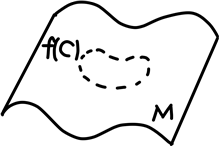
\includegraphics{2.png}
\caption{특이점이 $C$ 내부에 존재하지 않는 곡면 $M$과 그 부분집합인 단순폐곡선 $C$의 상}
\end{figure}


Curved origami cutting 문제는 간단히 말하여 어떤 isometry $f$가 존재하여 평면 위의 곡선 $C$가 $f$에 의해 parametrized된 후에도 $f(C)$가 똑같은 평면 위에 있을 수 있는가, 즉 cutting이 가능한가를 묻는다. $C$를 단순폐곡선에 대하여 문제를 제한하자. $p$의 generator $\gamma _T$ 위에 있지 않은 점의 generator가 $\gamma _T$와 평행하지 않다면 두 직선의 교점은 서로 다른 두 방향에서의 곡률이 같으므로 구면형(umbilic) 점이 되고 모든 방향에 대하여 곡률이 0이 되어 곡면 $M$이 평면과 합동이 아니면 $f(C)$는 당연히 평면 위에 있을 수 없게 된다. 임의의 점에서의 generator가 모두 평행하고 곡면 $M$을 $\gamma_T$가 평행이동할 때의 자취로 해석하더라도 평면 위의 단순폐곡선 $C$가 곡면 $M$의 매개변수변환이 취해진 후에 $f(C)$를 포함하는 평면이 ${\mathbb R}^3$에 존재하기 위하여 $C$ 위의 점의 generator들의 집합은 평면을 이루므로 문제의 조건에 어긋난다. 따라서 $f$에 Theorem 1.2.가 성립하지 않는 미분불가능한 특이점이 존재해야 하며 그 위치가 $C$의 내부여야 함은 $f(C)$가 평면 위에 있어야 함을 이용해 증명할 수 있다. 이 때 특이점의 역할은 generator의 진행을 막는 것으로 볼 수 있다. 곡면 $M$을 이 점에 대해서만 $f$가 미분불가능인 것으로 미분동형사상인 isometry의 조건을 완화시키는 것으로 약속하자. 폐곡선 $C$에 단순조건을 붙이는 이유는 flat-foldability에 대한 네 번째 공리와 대응하여 곡면이 자기 자신을 뚫지 못하게 하기 위함이므로 뚫고 지나가는 것이 아니라면 자기 자신과 만나는 것은 가능함을 기억해두자.


\begin{figure}
\centering
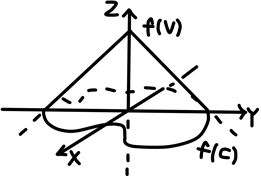
\includegraphics{3.png}
\caption{Single-vertex의 구조}
\end{figure}


우리는 이번 연구에서 특히 vertex라 정의할 특이점이 단순폐곡선 $C$ 내부에서 하나만 존재할 경우를 중점적으로 다루고자 한다. 이것은 flat-foldability 중 local flat-foldability에 대응되는 것이다. vertex가 하나인 문제에서 어떤 generator가 vertex를 향하지 않는다면 generator 사이의 교점이 생기지 않게 하기 위하여 임의의 두 generator는 평행을 이루며 특이점의 의미는 없어져 특이점을 가정하지 않은 본래의 상황으로 귀결되므로 모든 generator가 vertex에서 뻗어나간다고 할 수 있다. 이 사실은 $f(C)$를 밑면으로 하고 꼭짓점이 $f(V)$인 뿔(generalized cone)을 떠올릴 수 있게 한다. 이 뿔을 생각함으로써 얻을 수 있는 가장 큰 이점은 flat-foldability에 관한 Lemma 1.1. 을 3차원으로 일반화시키기가 매우 쉽다는 것이다.


\begin{figure}
\centering
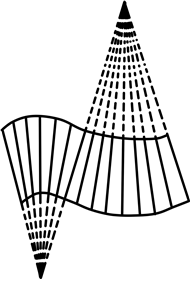
\includegraphics{4.png}
\caption{특이점이 $M$밖에 여러 개 있는 경우}
\end{figure}


vertex가 여러 개 있는 경우의 문제를 생각해본다면 generator들이 한 점에서 모여야 한다는 성질을 생각하여 특이점이 곡면 $M$ 밖에 있을 때 곡면 $M$에 속한 generator들을 여러 구간으로 나눈 후 각 구간에 포함된 generator들이 $M$ 밖의 한 점에서 모이게끔 할 수 있으며 곡면 $M$ 안에 있을 때는 특이점이 불연속적으로 분포할 수 없어 특이점들로 이루어진 곡선에 대하여 연구해 보아야 한다.







\section{Single-vertex Curved Origami Cutting의 해결}
\subsection{Parametrization $f$의 해석}


Single-vertex구조에서 $f(C)$를 밑면으로 하고 $f(V)$를 꼭짓점으로 하는 뿔의 모선 위에 있는 점들의 집합은 곡면 $M$에 포함된 닫힌 연결집합이다. 우리는 등거리사상 $f$의 성질을 파악하기 위하여 유클리드 평면 위에서 위의 $C$ 내부의 꼭짓점 $V$를 원점으로 하는 극좌표 $(r,\theta )$를 만들고 구간 $[0,2\pi)$에서 뿔의 모선에 해당하는 길이를 크기로 가지는 벡터로 가는 단사함수 $C(\theta)$로 둠으로써 $C(\theta)$의 그래프가 곡선 $C$를 그리게끔 하자. %그러면 $C$를 picecwise $C^2$함수로 가정했을 때 간단한 구분구적법의 아이디어로 $C$ 내부는 $C(\theta)$와 $C(\theta+d\theta)$와 $dC$를 세 변으로 하는 미소삼각형 들로 쪼갤 수 있다. $C$가 미분불가능한 함수라도 연속함수이므로 $C^2$함수로 근사시킴으로써 같은 방법으로 $C$를 다룰 수 있다.
%$C$를 $C^2$함수라고 가정하였으므로 $dC/d\theta$는 미분가능하고 $d\theta/dC$는 무한점 이외에는 연속이다. 그러나 $d\theta/dC$가 무한으로 발산함은 $C(\theta)$가 0으로 수렴함을 의미하므로 $d\theta/dC$의 부호가 바뀌는 것은 $C$가 원점 $V$를 지남을 뜻한다.
\\
\\
\\
\\
 따라서 $\theta$가 $d\theta$만큼 증가하면서 $C$ 위의 점이 그리는 자취의 미소길이를 나타내는 벡터 $dC(\theta)$에 대하여 $dC$가 $d\theta$에 대해 역행함으로써 $d\theta/dC$의 부호가 뒤바뀌는 경우, 즉 $C$를 단사함수로 둘 수 없는 경우는 생각하지 않는다.
이 때 parametrization $f$는 $V$를 $z$방향으로 이동시키고 이때 $C$를 분할하는 미소삼각형들이 합동변환을 유지하면서 $dC$의 $z$성분이 계속 0이 되게끔 평면을 곡면 $M$으로 바꾸는 사상으로 새로 정의하게 된다. $V$가 이동한 변위의 크기를 $z$라 할 때 아래 그림 5는 $f$를 취하기 전과 후의 미소삼각형의 변화를 나타낸 것이다.


%z방향에 대한 설명
%f(C)의 극좌표도 설명
%벡터f(C)


\begin{figure}
\centering
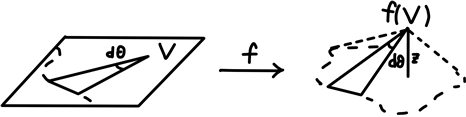
\includegraphics{5.png}
\caption{$f$에 의한 삼각형의 위치변화}
\end{figure}


각 $f(d\theta)$를 $xy$평면에 정사영시키는 함수를 $\pi \circ f^{-1}$라 할 때 $\pi(d\theta)$의 $d\theta$에 대한 비율은 $\theta$에 대한 함수로 나타낼 수 있으며 2절과 3절에서 더 자세히 다룰 것이지만 간단히 말하여 우리의 문제는 $\int_0^{2\pi}\pi(d\theta)$의 값이 $2\pi$ 또는 0이 되어야 하는 $f$의 존재성을 묻는 것이므로 $\pi(d\theta)$의 성질을 살펴볼 필요가 있다. 특히 $\pi(d\theta)$가 $z$에 대하여 증가하는지 감소하는지에 관한 문제는 본 문제의 해결에 있어 굉장히 큰 역할을 한다.


\begin{figure}
\centering
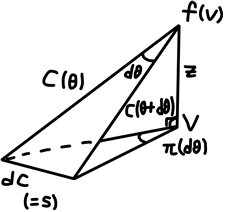
\includegraphics{6.png}
\caption{$d\theta$와 $d\theta'$의 관계}
\end{figure}


제 2 코사인법칙에 의하여 $\pi$를 수식으로써 정의할 수 있다.


\begin{eqnarray}
(dC)^2 & =& C(\theta)^2+C(\theta+d\theta)^2-2C(\theta)C(\theta+d\theta)\cos d\theta \nonumber
\\& =& C(\theta)^2 -z^2 +C(\theta+d\theta)^2 -z^2
-2\sqrt{(C(\theta)^2 -z^2)(C(\theta+d\theta)^2 -z^2)}\cos \pi (d \theta) \nonumber
\end{eqnarray}
\begin{equation}
\therefore \pi(d\theta)= \cos^-1 \left( \frac{C(\theta)C(\theta+d\theta)\cos d\theta -z^2}{\sqrt{(C(\theta)^2 -z^2)(C(\theta+d\theta)^2 -z^2)}} \right)
\end{equation}
\\

$\cos d\theta$를 상수로 보고 $\cos \pi(d\theta)$를 $z$의 함수로 보아 미분하면 $z$가 증가할 때 $\cos \pi (d\theta)$가 증가하는지 감소하는지 조건을 구하는 것이 가능하며 식은 다음과 같다.


\begin{equation}
\frac{\partial \cos\pi(d \theta)}{\partial z}(0)=0 \nonumber
\end{equation}

\begin{equation}
\frac{\partial \cos\pi(d \theta)}{\partial z}(0)>0 \iff 
C(\theta)^2 + C(\theta+d\theta)^2 > \frac{2C(\theta)C(\theta+d\theta)}{\cos d\theta} \nonumber
\end{equation}



위 식을 고전기하의 관점으로 분석해보자. $\theta$가 $d\theta$만큼 증가하면서 $C$ 위의 점이 그리는 자취의 길이, 즉 미소삼각형의 밑변을 $s$라 하면 $f$에 의한 미소삼각형의 변화는 $s$를 회전축으로 적당히 회전시킨 후 평행이동 및 $z$축을 회전축으로 한 회전이동을 한 것으로 볼 수 있다. $s$는 $C(\theta)$와 $C(\theta+d \theta)$가 가리키는 두 점을 이은 선분이므로 벡터 $dC$와 평행하고 크기가 같다.


\begin{figure}
\centering
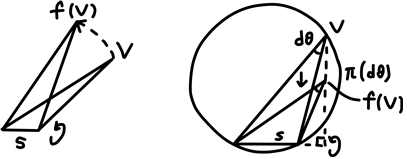
\includegraphics{7.png}
\caption{$d\theta$의 사영의 고전기하적 의미}
\end{figure}


정사영된 각 $\pi (d \theta)$의 크기에 영향을 미치는 것은 $s$에 대한 회전뿐이므로 이에 대한 것만 보자면 $z$가 증가할 때 $V$가 $s$에 수직하는 직선의 방향을 따라 $s$ 쪽으로 다가온다고 볼 수 있게 되므로 $z$가 0에서 증가할 때 $C(\theta)$, $C(\theta+d\theta)$, $s$가 이루는 삼각형의 외심과 $s$ 사이의 거리가 $V$와 $s$ 사이의 거리보다 작을 때 $d\theta <|\pi(d\theta)|$가 된다. 외접원의 크기와 원주각의 크기의 관계를 통해 어렵지 않게 증명할 수 있다. 실제로 어느 정도의 계산을 거치면 이계미분을 통해 구한 결과와 일치함을 보일 수 있다. $d\theta$를 0으로 수렴시키면 $C(\theta)$와 $C(\theta+d\theta)$ 사이의 각과 $s$ 또한 0으로 수렴하며 $z$가 0에서 증가할 때 $d\theta <|\pi(d\theta)|$일 필요충분조건을 다음과 같은 정리로 요약할 수 있다.

%Proposition
\begin{theorem}
$z$가 0에서 증가할 때 $d\theta <|\pi(d\theta)|$일 필요충분조건은 $C(\theta)$와 $s$ 사이의 각이 $\pi /4$보다 큰 것이다.
\end{theorem}


\subsection{Single-vertex cutting의 재조명}

다음과 같이 $f(C)$의 형태를 결정하는 과정을 생각하자:

$C$는 $\theta=0$에서부터 $\theta$를 $d\theta$만큼 증가시키면서 두 벡터 $C(\theta)$와 $C(\theta+d\theta)$의 차로 $s$를 결정함으로써 귀납적으로 $s$의 집합이 된다고 정의할 수 있다. 마찬가지로 $f(C)$ 또한 같은 평면 위에 $f(s)$를 두기 위하여 $\theta$를 $d\theta$만큼 증가시키면서 사이의 각도가 $\pi(d\theta)$이고 크기가 각각 두 벡터 $\sqrt{C(\theta)^2 -z^2 }$와 $\sqrt{C(\theta+d\theta)^2 -z^2 }$의 차로 $f(s)$를 결정함으로써 귀납적으로 정의할 수 있다.


\begin{theorem}
$C$와 $f(C)$가 똑같은 평면에 포함될 수 있을 필요충분조건은 $\int_0^{2\pi} \pi(d\theta)$의 절댓값이 $2\pi$, 0 중 하나인 것이다.
\end{theorem}

\begin{proof}
$C$의 정의역을 $2\pi$가 주기가 되게끔 실수 전체로 확장시켜 생각하면 $C$가 폐곡선일 필요충분조건은 $C(0)=C(2\pi)$이고 $f(C)$도 $C$와 같이 극좌표를 잡아 만든 그래프로 본다면 $f(C)$가 폐곡선이기 위한 필요충분조건은 두 조건
$$f(C)\left(\int_0^0 \pi(d\theta) \right)=f(C)(0)=f(C)\left(\int_0^{2\pi} \pi(d \theta)\right)$$
과 0과 $2\pi$가 평면에서 같은 위치를 나타내는 것처럼
$$\int_0^0 \pi(d\theta) =0 \equiv \int_0^{2\pi} \pi(d\theta) \quad \pmod {2\pi}$$
을 모두 만족하는 것이다. 이 때 $f(C)$가 각에서 벡터로 가는 함수임을 상기시키자. 위의 두 조건은 각각 의 값이 $\int_0^{2\pi} \pi(d\theta)$의 정수배임이 $C$와 $f(C)$가 같은 평면에 포함될 수 있을 충분조건과 필요조건임을 증명한다.
$\int_0^{2\pi} \pi(d\theta)$의 절댓값이 $4\pi$ 이상이면 $f(C)$이 단순하지 않으므로 본 명제가 성립한다.
\end{proof}


\begin{figure}
\centering
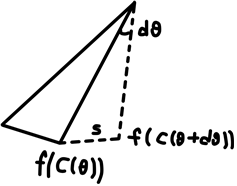
\includegraphics{8.png}
\caption{$f(C)$의 귀납적 결정}
\end{figure}


위 정리에서 적분값이 0인 경우는 $f(V)$를 $xy$평면에 정사영시킨 점이 $f(C)$ 외부에 있음을 뜻한다. Theorem 3.2.(정리4)는 다시 말해 $C$와 $f(C)$가 같은 평면 위에 있기 위한 충분조건이 $\pi$를 취한 후에 있어서도 적분값이 $2\pi$로 변하지 않는 것임을 밝힌다.
잠시 $d\theta/dC$의 부호가 바뀌는 문제로 돌아가 보자. $d\theta/dC$의 부호가 바뀌기 위하여 $d\theta/dC=0$인 점이 존재하는데 Theorem 3.2.(정리4)의 증명에서처럼 $dC$를 귀납적으로 정의함으로써 $C$와 $f(C)$를 결정하는 모델에서 이 점의 존재성은 $z$의 값으로 0보다 큰 수를 잡을 수 없게 한다. 이를 넓혀 생각하면 $z$의 범위에 대한 다음 식이 성립한다.


\begin{equation}
\sup(z)=\inf \left\{ C(\theta)^2 \frac{d\theta}{dC} : \theta \in [0,2\pi) \right\} \nonumber
\end{equation}




\subsection{Kawasaki's Theorem의 확장에 의한 해결}


Theorem 3.2.(정리4)에 따라 $\int _0 ^{2\pi} d \theta=\int _0 ^{2\pi} \pi(d \theta)$를 만족하기 위하여 가능한 것은 $d\theta<\pi(d\theta)$를 만족하는 $\theta$와 $d\theta>\pi(d\theta)$를 만족하는 $\theta$의 적절한 분포에 의한 것이다. 그러나 직관적으로 모든 $\theta$에 대하여 $d\theta<\pi(d\theta)$가 성립하는 곡선 $C$는 Proposition 3.1.(정리3)을 따라 대표적으로 원을 포함하여 무수히 많다. 이러한 곡선 $C$의 cutting이 가능한가의 여부를 Kawasaki's theorem의 아이디어로 접근하려 한다. 만약 $\forall \theta, d\theta<\pi(d\theta)$에서 cutting이 가능하다면 그렇지 않은 경우에도 cutting이 가능함은 자명하다.
$f(C)$의 귀납적 결정 모델을 다시 생각하자. $f(s)$를 결정하는 변수는 $C(\theta), \|C(\theta+d\theta)\|, |\pi(d\theta)|$로 엄밀히 말하여 $f(s)$가 단 하나 결정되지 않음을 파악해야 한다. 미소삼각형의 합동변환이라는 조건만 성립하면 되므로 $\pi(d\theta)$는 $\pi$를 취한 후 절댓값만 같다면 부호가 바뀌어도 문제가 되지 않는다는 것이다. 따라서 $f(s)$는 $\pi(d\theta)$의 부호에 따라 $C(\theta)$에 대칭이고 길이가 같은 두 가지 선분 중 하나로 결정되며 $\theta$에 따른 무수히 많은 기로에서 어느 것을 택하는가에 상관없이 $\int_0^{2\pi} \pi(d\theta)=2\pi$를 만족하게 하면 cutting은 가능하다. $\pi(d\theta)$의 부호선택과 $f(s)$의 반전에 대하여 구간 $[0,2\pi)$을 홀수 개의 구간으로 적절히 분할한 후 짝수 번째 구간의 $\pi(d\theta)$의 부호를 음으로 둠으로써 기술하도록 하자. (1)에서 볼 수 있다시피 $\pi(d\theta)$는 $\cos^{-1}$로 표현되는 다가함수이다. 단, $\pi(d\theta)$의 부호가 바뀌면서 깨질 수 있는 $f(C)$의 단순조건을 고려해야 한다.


\begin{figure}
\centering
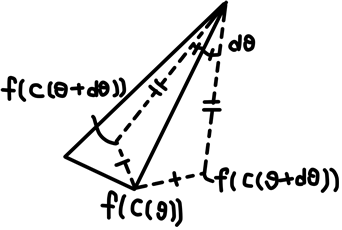
\includegraphics{9.png}
\caption{$\pi(d\theta)$의 부호 결정}
\end{figure}


$f(C)$의 단순성에 관한 문제를 다음과 같이 바꿔보자:


적분을 가시화하기 위해 $\theta \in [0,2\pi)$ 구간에서 $\theta \to |\pi(d\theta)|/d\theta$ 그래프를 그리고 그림과 같이 적절히 구간을 분할한 후 짝수 번째 구간에서 음의 적분을 하는 것을 생각하자. 짝수 구간에서 음의 적분은 해당하는 부분구간의 그래프를 연속을 유지한 채 뒤집는 것으로 해석할 수 있고 가로축의 총 적분구간이 짧아지지만 뒤집는 시행을 거친 후의 그래프 내부의 넓이를 바로 재는 것으로 적분이 자연스레 구해질 수 있다. 이 그래프에서 $f(C)$의 단순성은 그래프 $\theta \to |\pi(d\theta)|/d\theta$의 단순성과 동치이다.

모든 $\theta$에 대하여 $d\theta<|\pi(d\theta)|$이면 (1)에서 $|\pi(d\theta)|/d\theta)$는 $z$에 대한 증가함수이고 $\theta$에 따른 $|\pi(d\theta)|/d\theta$의 증가상태 또는 감소상태는 $z$와 독립적이므로 다음과 같은 조건을 세워 다음 정리를 보자.


\begin{theorem}
적당한 양의 실수 $\varepsilon$이 존재하여 함수 $\frac{|\pi(d\theta)|}{d\theta}(z,\theta)$가 $z(<\varepsilon)$에 대한 증가함수이고 $\theta$에 대하여 nowhere monotonic이 아니면 적당한 $z(<\varepsilon)$와 단조구간 $[a,b) \subset [0,2\pi)$가 존재하여 $\theta$에 대해 적분한 다음 식이 성립한다.


\begin{equation}
\int_0 ^{2\pi}\pi(d\theta)=\int_0^{2\pi} |\pi(d\theta)|-2\int_{\frac{2a+b}3}^{\frac{a+2b}3}|\pi(d\theta)|=2\pi \nonumber
\end{equation}

\end{theorem}


\begin{figure}
\centering
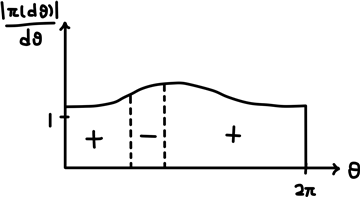
\includegraphics{10-1.png}
\end{figure}

\begin{figure}
\centering
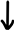
\includegraphics{10-2.png}
\end{figure}

\begin{figure}
\centering
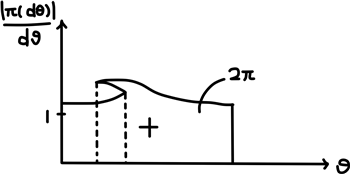
\includegraphics{10-3.png}
\caption{$\theta \to |\pi(d\theta)|/d\theta$그래프에서의 구간반전}
\end{figure}


\begin{proof}
$\frac{|\pi(d\theta)|}{d\theta} (z,\theta)$가 $\theta$에 대하여 nowhere monotonic이 아니므로 단조구간 $[a,b)$는 반드시 존재하며 또한 $z$에 대한 증가함수이므로 이것의 적분함수도 $z$에 대한 증가함수이고 다음과 같은 식을 얻는다.


\begin{equation}
\lim_{z\to 0} \frac{\pi(d\theta)}{d\theta} =1 \nonumber
\end{equation}
\begin{equation}
\lim_{z\to 0} \int_0^{2\pi} \pi(d\theta)=2\pi- \frac23 (b-a) <2\pi
\end{equation}


적당한 $\varepsilon$에 대하여 다음과 같이 양의 실수 $\phi$를 정의하자.

\begin{equation}
\lim_{z\to \varepsilon} \int_0^{2\pi} |\pi(d\theta)|-2\pi=\phi>0 \nonumber
\end{equation}


구간 $(a,b)$의 크기를 적당히 작게 잡으면 다음 식이 성립한다.

\begin{equation}
\lim_{z\to \varepsilon} \int_{\frac{2a+b}3}^{\frac{a+2b}3} |\pi(d\theta)|< \frac{\phi}2 \nonumber
\end{equation}

\begin{equation}
\lim_{z\to \varepsilon} \int _0^{2\pi} \pi(d\theta)=
\lim_{z\to \varepsilon} \left( \int _0^{2\pi} |\pi(d\theta)|-2\int_{\frac{2a+b}3}^{\frac{a+2b}3} |\pi(d\theta)| \right)>2\pi
\end{equation}


(2)과 (3)에 따라서 중간값의 정리에 의해 $\int_0^{2\pi} \pi(d\theta)=2\pi$를 만족하는 양의 실수 $z(<\varepsilon)$에 대하여 $[a,b)$가 존재한다. 
\end{proof}

구간 $[a,b)$가 단조구간일 때 구간 $[0,2\pi)$를 세 부분구간 $\left[0,\frac{2a+b}3\right), \left[\frac{2a+b}3,\frac{a+2b}3\right), \left[\frac{a+2b}3,2\pi\right)$로 분할한 후 구간 $\left[\frac{2a+b}3,\frac{a+2b}3\right)$에서의 $\pi(d\theta)$가 음수가 되도록 적분하면 Theorem 3.3.(정리5)에 의해서 $f(C)$의 단순성을 잃지 않고 cutting이 가능함을 알 수 있다.


\begin{figure}
\centering
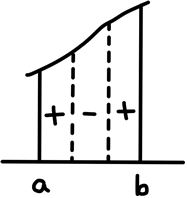
\includegraphics{11.png}
\caption{Theorem 3.3.의 의미}
\end{figure}


두 실수 $a<b \in (0,2\pi)$에 대하여 $|\pi(d\theta)|/d\theta$가 $\theta$에 대해 단조성을 가지는 구간 $[a,b)$들의 집합을 $K$라 하면 Theorem 3.3.을 만족하는 $z$와 구간 $[a,b)$에 대해 함수관계 $\varphi:K\to (0,\varepsilon)$를 정의할 수 있는데 $|\pi(d\theta)|$는 $z$와 $\theta$에 대해 모두 연속이므로 $\varphi$ 또한 연속이다. 따라서 다음과 같은 따름 정리를 얻는다.


\begin{corollary}
$z$가 연속적으로 증가하여 $V$가 $f(V)$에 도달할 때 곡선 $C$ 또한 $xy$평면에 포함된 상태를 유지하며 연속적 변환을 거쳐 $f(C)$에 도달할 수 있다.
\end{corollary}

\section{결론}
평면 $P$ 위의 nowhere monotonic이 아닌 piecewise $C^2$ 단순폐곡선 $C$ 내부에 한 점 $V$를 잡아 $V$를 지나는 임의의 직선이 $C$에 접하지 않고 $C$와의 교점이 두 개일 때 $f(C)\subset P$를 만족하고 $V$를 유일한 vertex로 하는 curved origami를 나타내는 곡면 $M$의 parametrization $f:P\to M$가 연속적으로 분포한다.



\bibliographystyle{plain}
\bibliography{human}









\end{document}




